\begin{frame}[t]{World Model Architectures: Generative vs.\ Joint Embedding}
  \centering
  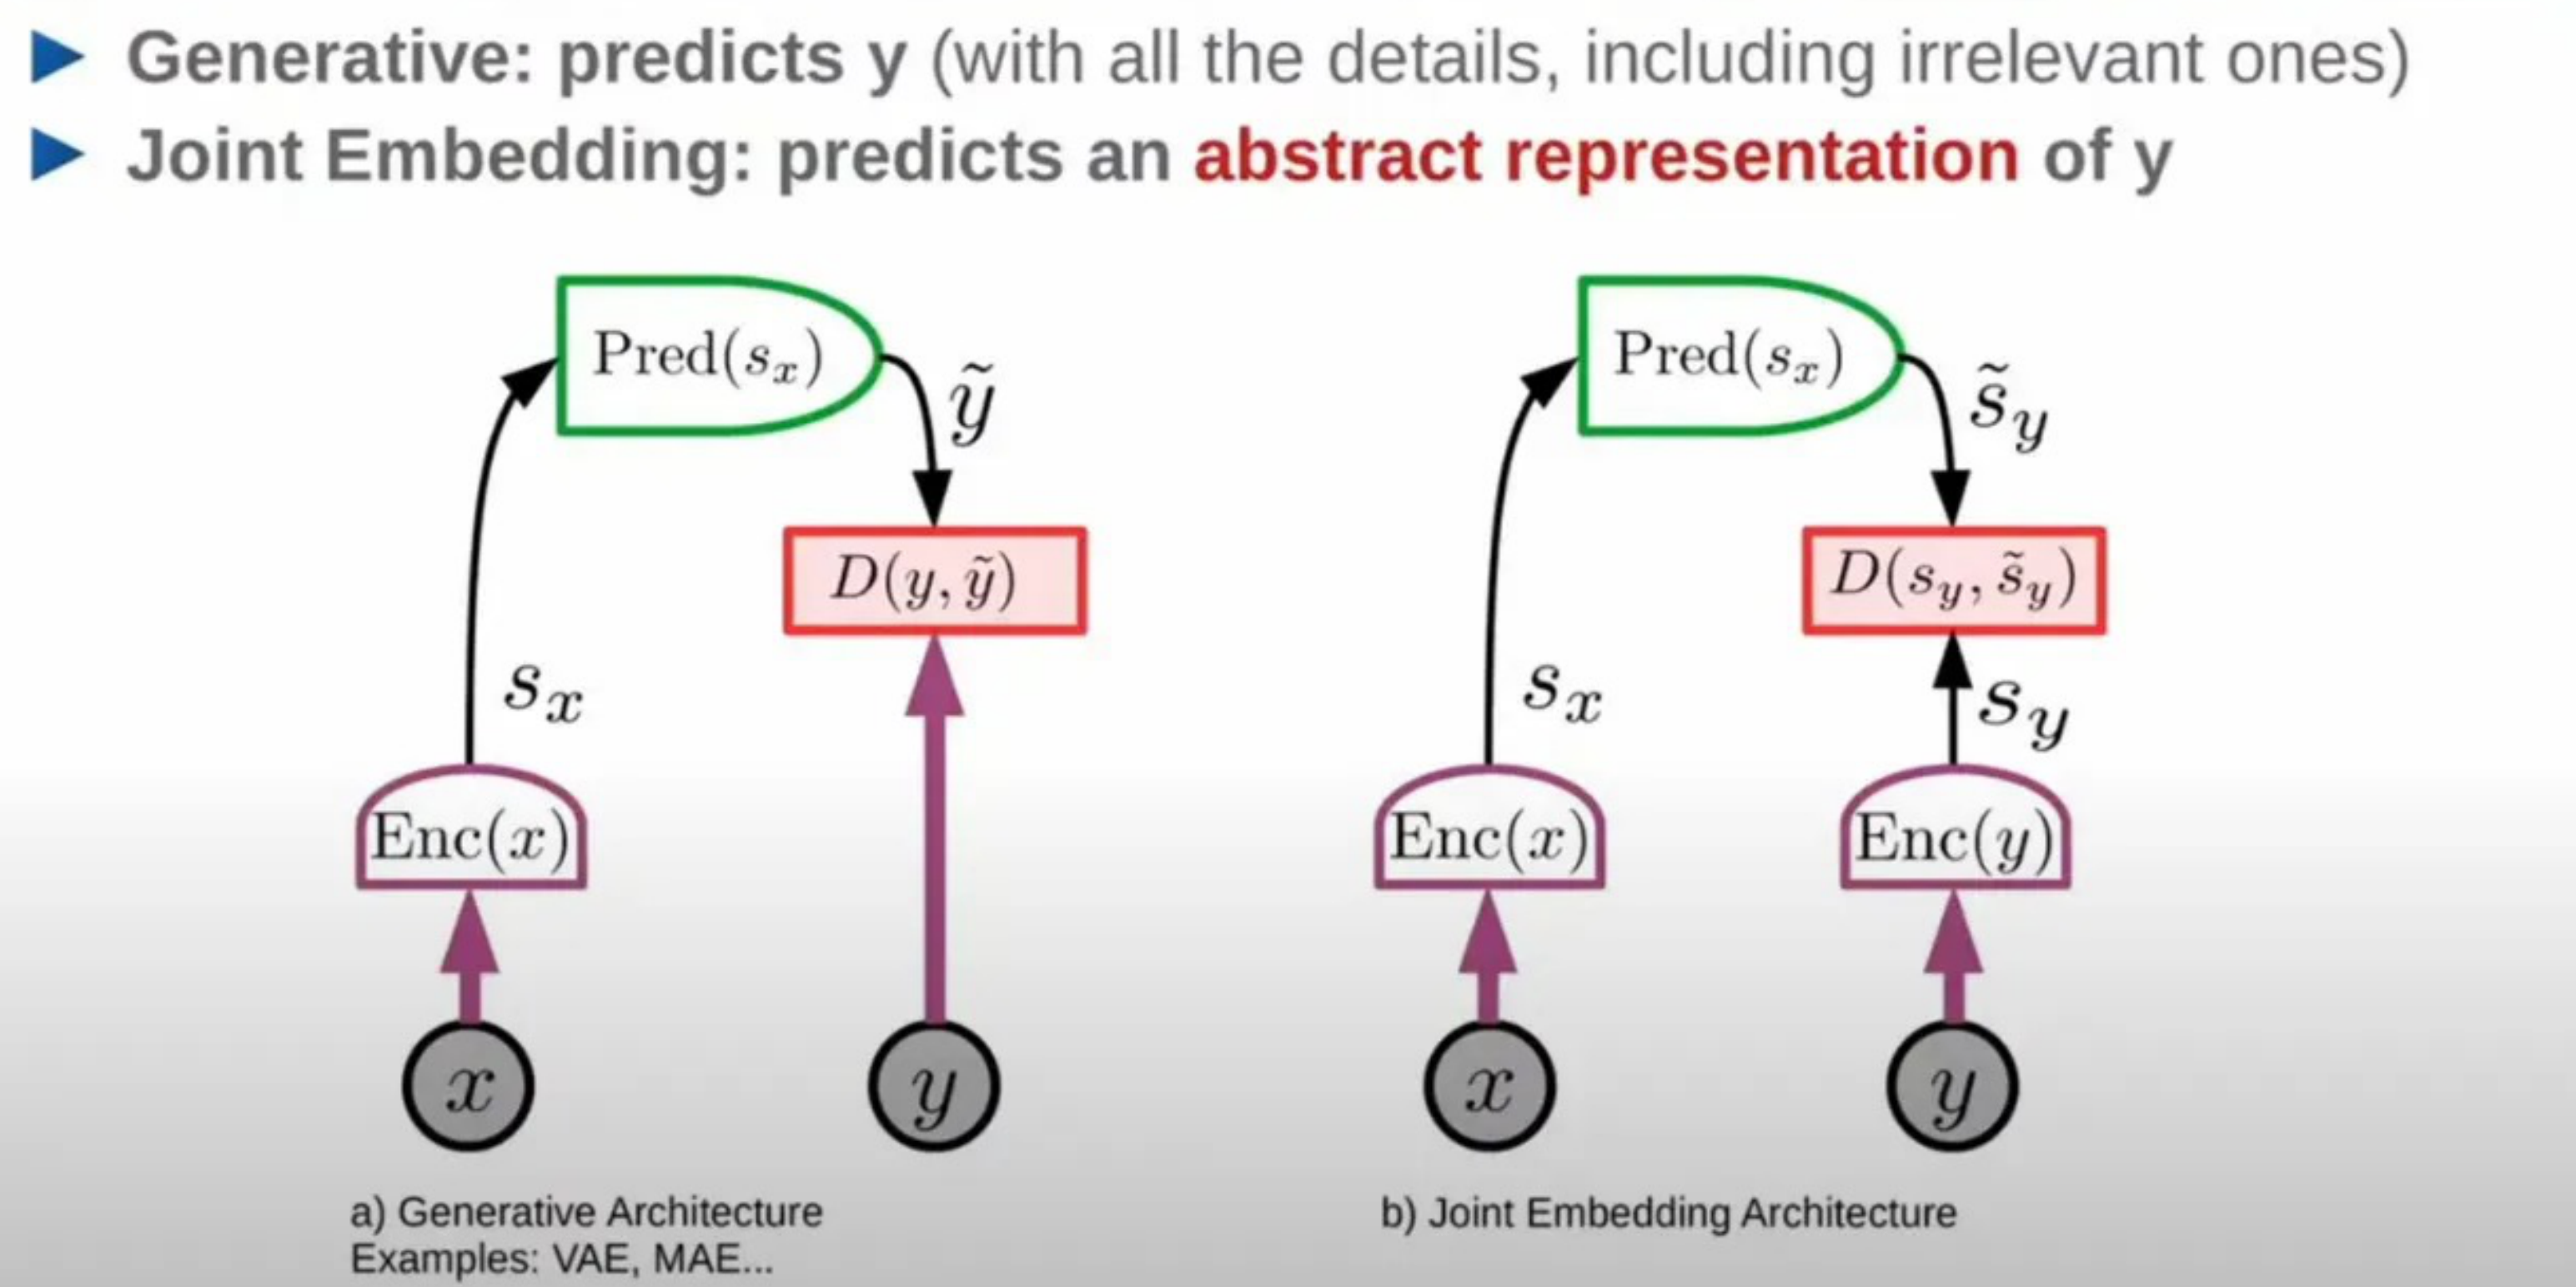
\includegraphics[width=\linewidth,height=0.82\textheight,keepaspectratio]{images/world-models/jepa_cs25_sl05_lecun_world_model_figure.png}\\[0.08em]
  {\scriptsize Image credit: \href{https://drive.google.com/file/d/1bF5Yfzf-FG5iNIAgsXn2DwVD3l3ymvZW/view}{CS25}.}
\end{frame}

\begin{frame}{How Could We Use a World Model?}
  \centering
  \vspace{0.1em}
  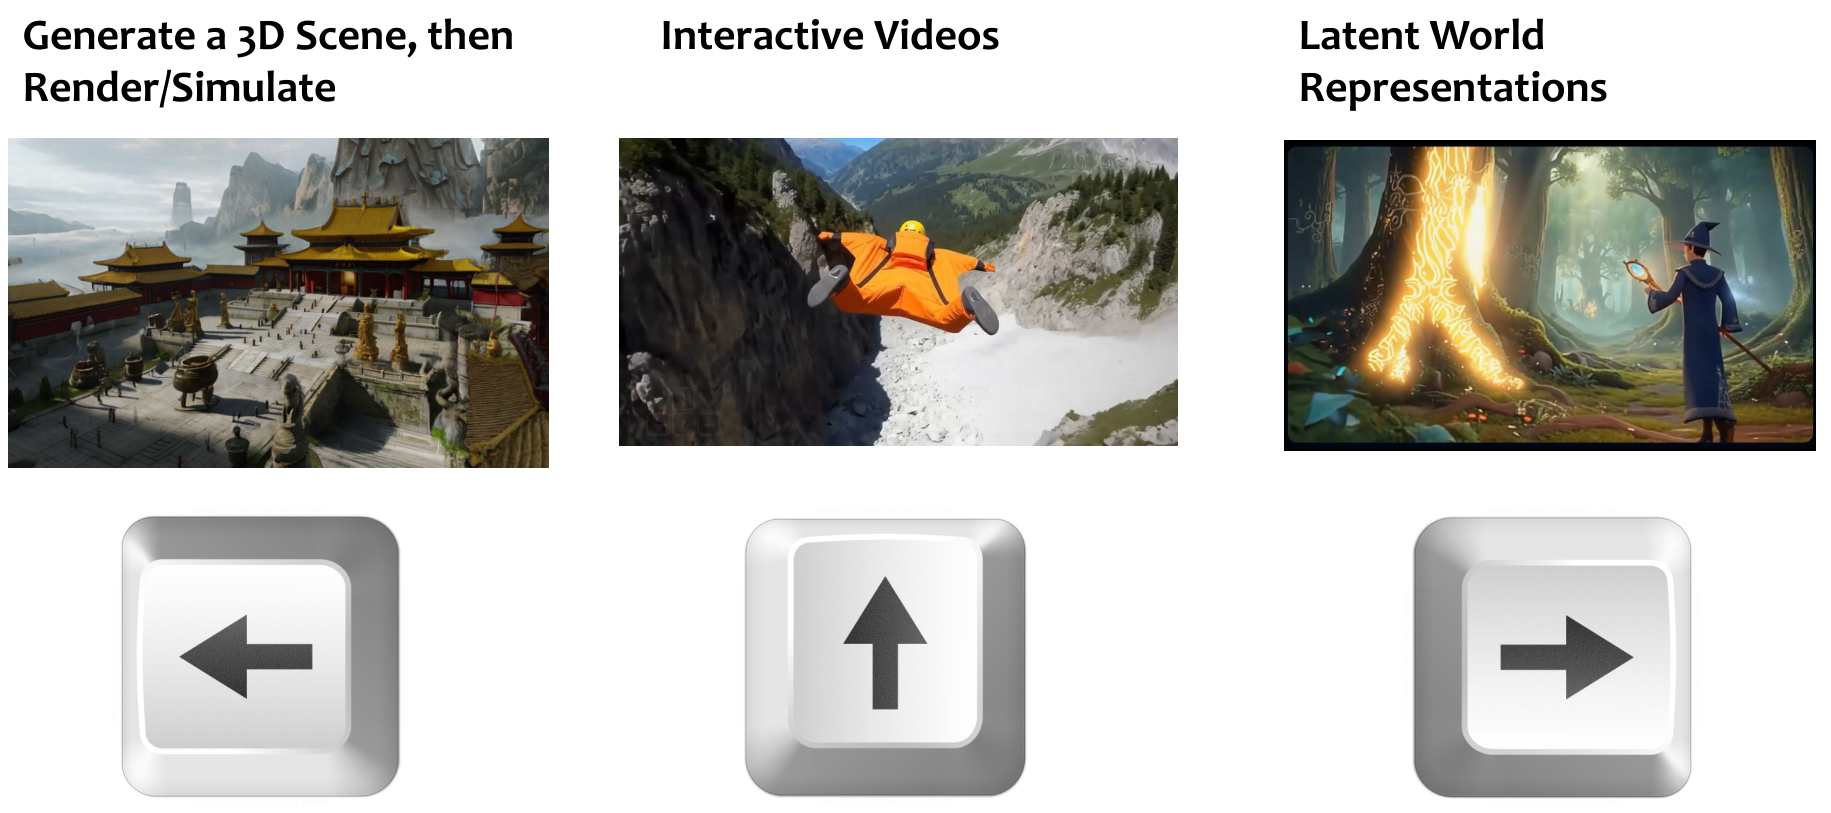
\includegraphics[width=\linewidth,height=0.88\textheight,keepaspectratio]{images/world-models/cmu10423_lecture26_world_models_slide10.png}\\[0.32em]
  {\scriptsize CMU 10-423, Lecture 26.}
\end{frame}

\begin{frame}[t]{Generative World Models}
  \centering
  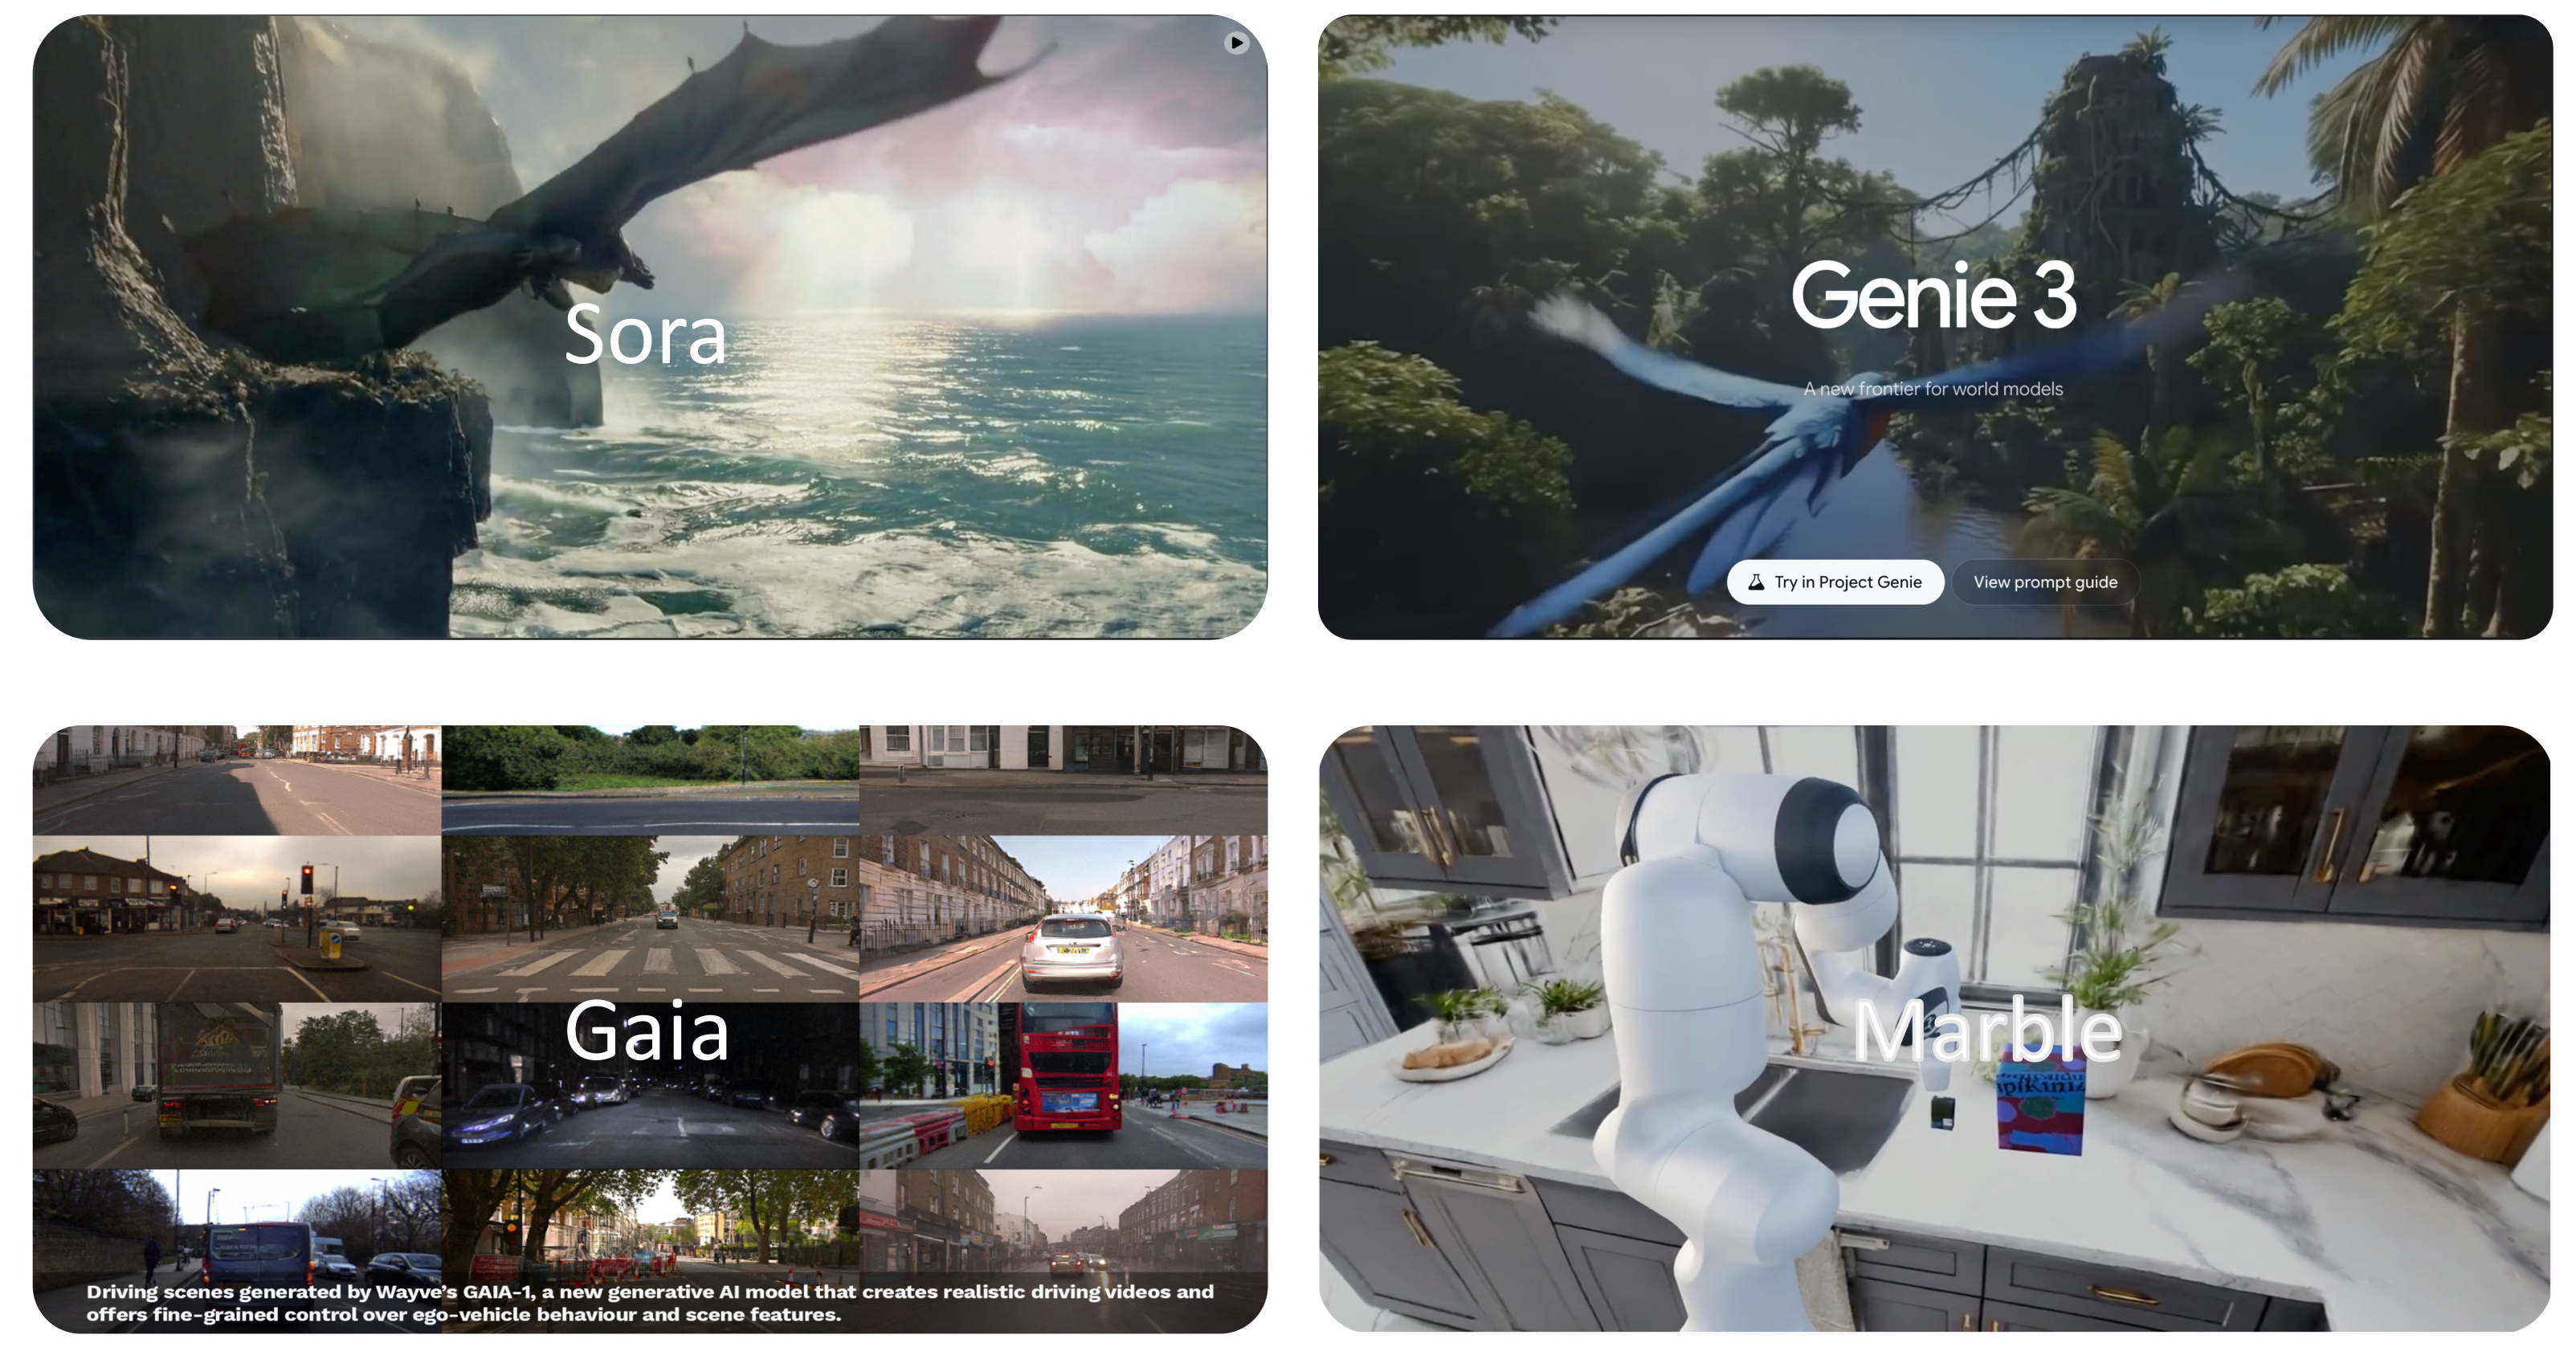
\includegraphics[width=0.76\linewidth,height=0.86\textheight,keepaspectratio]{images/world-models/jepa_cs25_sl04_generative_world_models_sora_gaia.png}\\[0.04em]
  {\scriptsize Image credit: \href{https://drive.google.com/file/d/1bF5Yfzf-FG5iNIAgsXn2DwVD3l3ymvZW/view}{CS25}.}
\end{frame}
